%%%%%%%%%%%%%%%%%%%%%%%%%%%%%%%%%%%%%%%%%
% Short Sectioned Assignment LaTeX Template Version 1.0 (5/5/12)
% This template has been downloaded from: http://www.LaTeXTemplates.com
% Original author:  Frits Wenneker (http://www.howtotex.com)
% License: CC BY-NC-SA 3.0 (http://creativecommons.org/licenses/by-nc-sa/3.0/)
%%%%%%%%%%%%%%%%%%%%%%%%%%%%%%%%%%%%%%%%%

% \documentclass[paper=a4, fontsize=11pt]{scrartcl} % A4 paper and 11pt font size
\documentclass[11pt, a4paper]{book}
\usepackage[T1]{fontenc} % Use 8-bit encoding that has 256 glyphs
\usepackage[utf8]{inputenc}
\usepackage{fourier} % Use the Adobe Utopia font for the document - comment this line to return to the LaTeX default
\usepackage{listings} % para insertar código con formato similar al editor
\usepackage[spanish, es-tabla]{babel} % Selecciona el español para palabras introducidas automáticamente, p.ej. "septiembre" en la fecha y especifica que se use la palabra Tabla en vez de Cuadro
\usepackage{url} % ,href} %para incluir URLs e hipervínculos dentro del texto (aunque hay que instalar href)
\usepackage{graphics,graphicx, float} %para incluir imágenes y colocarlas
\usepackage[gen]{eurosym} %para incluir el símbolo del euro
\usepackage{cite} %para incluir citas del archivo <nombre>.bib
\usepackage{enumerate}
\usepackage{hyperref}
\usepackage{graphicx}
\usepackage{tabularx}
\usepackage{booktabs}

\usepackage[table,xcdraw]{xcolor}
\hypersetup{
	colorlinks=true,	% false: boxed links; true: colored links
	linkcolor=black,	% color of internal links
	urlcolor=cyan		% color of external links
}
\renewcommand{\familydefault}{\sfdefault}
\usepackage{fancyhdr} % Custom headers and footers
\pagestyle{fancyplain} % Makes all pages in the document conform to the custom headers and footers
\fancyhead[L]{} % Empty left header
\fancyhead[C]{} % Empty center header
\fancyhead[R]{Miguel Ángel Posadas Arráez} % My name
\fancyfoot[L]{} % Empty left footer
\fancyfoot[C]{} % Empty center footer
\fancyfoot[R]{\thepage} % Page numbering for right footer
%\renewcommand{\headrulewidth}{0pt} % Remove header underlines
\renewcommand{\footrulewidth}{0pt} % Remove footer underlines
\setlength{\headheight}{13.6pt} % Customize the height of the header

\usepackage{titlesec, blindtext, color}
\definecolor{gray75}{gray}{0.75}
\newcommand{\hsp}{\hspace{20pt}}
\titleformat{\chapter}[hang]{\Huge\bfseries}{\thechapter\hsp\textcolor{gray75}{|}\hsp}{0pt}{\Huge\bfseries}
\setcounter{secnumdepth}{4}
\usepackage[Lenny]{fncychap}

\usepackage{cite} %para incluir citas del archivo <nombre>.bib
\usepackage{apacite}
\hypersetup{%
	citecolor=black
}

% Para las tablas
\usepackage{array}
\usepackage{colortbl}
\usepackage{multirow}
\usepackage{adjustbox}

\usepackage{fancyvrb}
\usepackage{color}

\definecolor{dkgreen}{rgb}{0,0.6,0}
\definecolor{gray}{rgb}{0.5,0.5,0.5}
\definecolor{mauve}{rgb}{0.58,0,0.82}

\newcommand*{\Comment}[1]{\makebox[10cm][l]{#1}}%

\lstset{frame=tb,
  language=Matlab,
  aboveskip=3mm,
  belowskip=3mm,
  showstringspaces=false,
  columns=flexible,
  basicstyle={\small\ttfamily},
  numbers=none,
  numberstyle=\tiny\color{gray},
  keywordstyle=\color{blue},
  commentstyle=\color{dkgreen},
  stringstyle=\color{mauve},
  breaklines=true,
  breakatwhitespace=true,
  tabsize=2,
  numbers=left,
  xleftmargin = 5mm,
  escapechar=\&% char to escape out of listings and back to LaTeX
}


\begin{document}

	% Plantilla portada UGR
	\begin{titlepage}
\newlength{\centeroffset}
\setlength{\centeroffset}{-0.5\oddsidemargin}
\addtolength{\centeroffset}{0.5\evensidemargin}
\thispagestyle{empty}

\noindent\hspace*{\centeroffset}\begin{minipage}{\textwidth}

\centering

\includegraphics[width=0.9\textwidth]{logos/logo_ugr.jpg}\\[1.4cm]

\textsc{ \Large TRABAJO FIN DE GRADO\\[0.2cm]}
\textsc{ GRADO EN INGENIERÍA INFORMÁTICA}\\[1cm]

{\Huge\bfseries Programación eficiente de un algoritmo de procesamiento de la actividad cerebral \\}
\noindent\rule[-1ex]{\textwidth}{3pt}\\[3.5ex]
{\large\bfseries Implementación y optimización mediante paralelización de un algoritmo de análisis fractal de matrices binarias }
\end{minipage}

\vspace{1cm}
\noindent\hspace*{\centeroffset}
\begin{minipage}{\textwidth}
\centering

\textbf{Autor}\\ {Miguel Ángel Posadas Arráez}\\[2.5ex]
\textbf{Director}\\ Juan Ruiz de Miras\\[2cm]

\includegraphics[width=0.3\textwidth]{logos/etsiit_logo.png}\\[0.1cm]
\textsc{Escuela Técnica Superior de Ingenierías Informática y de Telecomunicación}\\
\textsc{---}\\
Granada, Junio de 201x
\end{minipage}
\end{titlepage}


	% Plantilla prefacio UGR
	\thispagestyle{empty}

\begin{center}
{\large\bfseries Programación eficiente de un algoritmo de procesamiento de la actividad cerebral \\ Implementación y optimización mediante paralelización de un algoritmo de análisis fractal de matrices binarias }\\
\end{center}
\begin{center}
Miguel Ángel Posadas Arráez\\
\end{center}

%\vspace{0.7cm}

\vspace{0.5cm}
\noindent{\textbf{Palabras clave}: \textit{Box counting, análisis fractal de matrices binarias, programación paralela, programación GPU}
\vspace{0.7cm}

\noindent{\textbf{Resumen}\\
El procesamiento de datos es una parte esencial en el estudio de diversas enfermedades neurodegenerativas. No obstante, las técnicas actuales para la adquisión de estos datos(resonancia magnética, encefalografía etc...) generan grandes volumenes de datos, lo que conlleva que su procesamiento tenga un gran coste computacional. El propósito de este trabajo es la programación eficiente del método conocido como Box counting para el procesamiento de matrices binarias.  Para la toma de tiempos y con el objetivo de poder hacer diversas comparaciones hemos utilizado dos plataformas con software y hardware diferentes. En un principio, el algoritmo venía programado en Matlab, con el objetivo de obtener una versión más eficiente de este algoritmo implementé una versión secuencial en C++ y posteriormente traté de aprovechar el paralelismo dado por los procesadores multi-core introduciendo la tecnología OpenACC obteniendo aceleraciones de hasta 15.7x. Finalmente, para la obtención de mejores aceleraciones, utilizamos el paradigma de computación de propósito general en unidades de procesamiento gráfico (GPGPU) para aprovechar la arquitectura \textit{Single Instruction, Multiple Data} (SIMD) con el que obtenimos aceleraciones de hasta 77.47x .
	

\cleardoublepage

\begin{center}
	{\large\bfseries Efficient programming of a cerebral processing activity algorithm \\ Implemantation and optimization with parallelization of a binary matrixes fractal analysis algorithm }\\
\end{center}
\begin{center}
	Miguel Ángel Posadas Arráez\\
\end{center}
\vspace{0.5cm}
\noindent{\textbf{Keywords}: \textit{Box counting, Fractal dimension of binary matrix, parallel programming, GPU programming}
\vspace{0.7cm}

\noindent{\textbf{Abstract}\\
Data processing is essential in neurodegenerative diseases studies. However, the existing ways of getting this data (magnetic resonance, electro-encephalography ... ) generate big data volumes, so processing that data has a expensive computing cost. The purpose of this paper is the efficient programming of the Box counting method in order to apply it at binary matrixes processing. They have been used two differents hardware and software platforms to track the time and making comparisons between then. At first, the algorithm was write on Matlab. I \textit{"translated"} that code to C++ with the goal of getting a more efficient sequential algorithm. Then, I tried to parallelize it with OpenACC with the goal of using the multicore CPU and I get a 15.7x speedup. Finally, in order to get the best speedup, I used the general-purpose computing on graphics processing units (GPGPU) to take advantage of the \textit{Single Instruction, Multiple Data} (SIMD) architecture on the graphics processing unit (GPU), getting a speedup of 77.47x.



\cleardoublepage

\thispagestyle{empty}

\noindent\rule[-1ex]{\textwidth}{2pt}\\[4.5ex]

D. \textbf{Juan Ruiz de Miras}, Profesor del Departamento de Lenguajes y Sistemas Informáticos

\vspace{0.5cm}

\textbf{Informo:}

\vspace{0.5cm}

Que el presente trabajo, titulado \textit{\textbf{Programación eficiente de un algoritmo de procesamiento de la actividad cerebral}},
ha sido realizado bajo mi supervisión por \textbf{Miguel Ángel Posadas Arráez}, y autorizo la defensa de dicho trabajo ante el tribunal
que corresponda.

\vspace{0.5cm}

Y para que conste, expiden y firman el presente informe en Granada a Julio de 2021.

\vspace{1cm}

\textbf{El/la director(a)/es: }

\vspace{5cm}

\noindent \textbf{Juan Ruiz de Miras}

\chapter*{Agradecimientos}






	% Índice de contenidos
	\newpage
	\tableofcontents

	% Índice de imágenes y tablas
	\newpage
	\listoffigures

	% Si hay suficientes se incluirá dicho índice
	\listoftables 
	\newpage

	%Si hay suficientes incluir este 
	\lstlistoflistings

	\chapter{Introducción}


El cálculo de la dimensión fractal de un conjunto de datos es una técnica con una gran multitud de aplicaciones, desde el ámbito económico, -- incluyendo su relación con la premisa del Bitcoin --  {\cite{delfin2016fractal}}, hasta el campo de la medicina y estudio del cuerpo humano, siendo este cálculo útil en la detección de tumores cerebrales {\cite{iftekharuddin2009fractal}}.

La dimensión fractal tiene su cabida en la neurociencia, siendo útil para el procesamiento de la actividad cerebral con el fin de poder estudiar diversas patologías neurodegenerativas \cite{fernandez2001use}. Sin embargo las técnicas actuales para la adquisición de este tipo de datos tales como las electroencefalografías o las resonancias magnéticas, generan grandes volúmenes de datos que implican un alto coste computacional, ya que en función de la dimensión del conjunto de datos, el orden del algoritmo aumenta de manera exponencial, siendo O(n) para conjuntos de datos de una dimensión y O($n^{4}$)  para matrices de cuatro dimensiones.

El propósito de este proyecto es el de la implementación eficiente del algoritmo conocido como Box counting. Para ello, partiendo del algoritmo, inicialmente escrito en el lenguaje de programación Matlab se desarrolla una versión secuencial, escrita en C++ que sirve como base para utilizar diversas tecnologías,como OpenACC y CUDA, con el fin de aprovechar el paralelismo que proporcionan los microprocesadores actuales así como la arquitectura SIMD (\textit{Single Instruction Multiple Data}) presente en las tarjetas gráficas.
	
	\chapter{Plan de proyecto}

En este apartado se presenta la planificación seguida a lo largo de todo el proyecto. Se especifican una serie de tareas diferenciadas entre sí que a continuación serán detalladas en profundidad.\\ Para dar por finalizada una tarea, y así poder pasar a la siguiente, ésta ha debido ser revisada previamente por el tutor. \\ Dentro del plan de estudios de la titulación, el trabajo de fin de grado tiene una carga de 12 créditos ECTS, y teniendo en cuenta que cada crédito ECTS equivale a 25 horas obtenemos, que el proyecto debe ser completado en 300 horas. De esta manera la planificación que procederemos a desarrollar en esta sección, se elabora considerando que el horario va a ser de lunes a viernes con jornadas de 3 horas de trabajo.\\

\section{Descripción de las tareas}
\subsection{Planificación del proyecto}
\label{tareaPlanificacion}
La planificación del proyecto corresponde a la primera tarea. Se subdivide el proyecto en las propias tareas que se están comentando en este punto, se realiza una estimación de tiempo de la que se genera un diagrama de Gantt que se puede consultar en la Figura \ref{fig:Gantt}, y una estimación de costos, que queda reflejada en la sección \ref{Costos}.\\

Se estima que esta tarea tendrá una duración de 5 horas.

\subsection{Estudio del algoritmo Box counting}
Con esta tarea se deja un tiempo para obtener formación sobre el algoritmo Box counting, conocer cómo funciona el \textit{"Fixed grid scan"}, y entender la implementación inicial escrita en Matlab. Para la realización de esta tarea se requiere de la adquisición de unas nociones básicas de Matlab debido al desconocimiento previo del lenguaje.\\

Se estima que esta tarea tendrá una duración de 10 horas.

\subsection{Implementación en C++ del algoritmo Box counting}
Una vez se haya comprendido el funcionamiento del algoritmo con el que se va a trabajar a lo largo de todo el proyecto, se procederá a su implementación secuencial en C++. Dentro de esta tarea, entra la comprobación de la corrección del código implementado, comprobando que es válido y funciona correctamente con datos reales de activación cerebral.\\

Se estima que esta tarea tendrá una duración de 10 horas.

\subsection{Experimentación y toma de tiempos del algoritmo sin paralelizar}
Se deja como tarea una etapa para la experimentación y toma de tiempos del algoritmo secuencial obtenido de la tarea anterior. Para la toma de tiempos se seguirá la metodología que se expone en el capítulo siguiente. El objetivo de la toma de tiempos del algoritmo secuencial es poder realizar comparaciones con las versiones que se implementen posteriormente, y medir que versión proporciona mejores aceleraciones.\\

Se estima que esta tarea tendrá una duración de 5 horas.

\subsection{Paralelización del algoritmo con OpenACC}
Se planifica una tarea que conlleva la búsqueda de bibliografía y el estudio del estándar de programación OpenACC. El objetivo de esto es poder añadir al código secuencial las directivas OpenACC necesarias para explotar el paralelismo que nos aporta el uso de una CPU multicore.\\

Se estima que esta tarea tendrá una duración de 70 horas.

\subsection{Experimentación y toma de tiempos de la paralelización con OpenACC}
Se planifica como tarea una etapa para la experimentación y toma de tiempos del código resultante de la tarea anterior. Además se analizarán los tiempos obtenidos y se compararán con los tiempos obtenidos en la etapa de experimentación del código secuencial mediante el cálculo de las aceleraciones.\\

Se estima que esta tarea tendrá una duración de 10 horas.

\subsection{Paralelización del algoritmo con CUDA}
Se planifica una tarea que conlleva la búsqueda de bibliografía y el estudio de la plataforma de programación CUDA. De esta manera, en esta fase del proyecto, se implementará todo lo necesario para aprovechar la computación de propósito general en unidades de procesamiento gráfico (GPGPU) para aprovechar las tarjetas gráficas de la compañía Nvidia.\\

La paralelización con CUDA es un poco más compleja que la paralelización con OpenACC, por tanto, para realizar esta tarea se empezará implementado la versión en 2D, y partiendo de esa versión como base, se desarrollarán la versión 3D y 4D.\\

Se estima que esta tarea tendrá una duración de 110 horas.

\subsection{Experimentación y toma de tiempos de la paralelización con CUDA}
Se deja como tarea una etapa para la experimentación y toma de tiempos del código resultante de la tarea anterior. Además se analizarán los tiempos obtenidos y se compararán con los tiempos obtenidos en la etapa de experimentación del código secuencial y con la etapa de experimentación del código paralelizado con OpenACC mediante el cálculo de las aceleraciones.\\

Se estima que esta tarea tendrá una duración de 20 horas.

\subsection{Análisis de los resultados obtenidos}
El objetivo de esta tarea, es dejar un tiempo para la comparación de todos los resultados obtenidos en las etapas de experimentación y toma de tiempos, así como discusión y redacción de conclusiones sobre los resultados obtenidos.\\

Se estima que esta tarea tendrá una duración de 20 horas.

\subsection{Elaboración de la memoria}
Durante el desarrollo de todo el proyecto se irá elaborando una memoria a modo de documentación del trabajo realizado, aunque se estiman 30 horas adicionales para terminarla.

\subsection{Preparación de la defensa ante el tribunal}
Tras la entrega del trabajo, se deja un tiempo para la elaboración del material necesario para la defensa y exposición del proyecto ante el tribubal.\\

Se estima que esta tarea tendrá una duración de 10 horas.


\section{Diagrama de Gantt}
Como anticipábamos en \textit{"\nameref{tareaPlanificacion}"}, la primera etapa del proyecto es la planificación temporal del mismo. Para ello el primer paso es la división del proyecto en tareas y su correspondiente especificación. A continuación, se realiza una estimación de los días necesarios que tomará cada tarea, teniendo en cuenta que se trabajará en jornadas de 3 horas diarias de lunes a viernes. Finalmente, se hace una planificación temporal de todas las tareas en base a la estimación de tiempo realizada, obteniendo así el diagrama de la Figura \ref{fig:Gantt}. En la tabla \ref{fig:Planificacion} se puede consultar la estimación de cada tarea así como, su fecha de inicio y finalización\\ Debido a la falta de experiencia en un proyecto de este tipo, esta especificación puede que no sea suficientemente detallada, en los siguientes capítulos se profundizará más en la descripción de las distintas tareas.\\ Esto es una planificación inicial del proyecto, como en todo proyecto es posible que surjan inconvenientes que retrasen alguna de las tareas o que se hayan subestimado alguna de ellas.
\newpage
\begin{figure}[h]
    \raggedright
    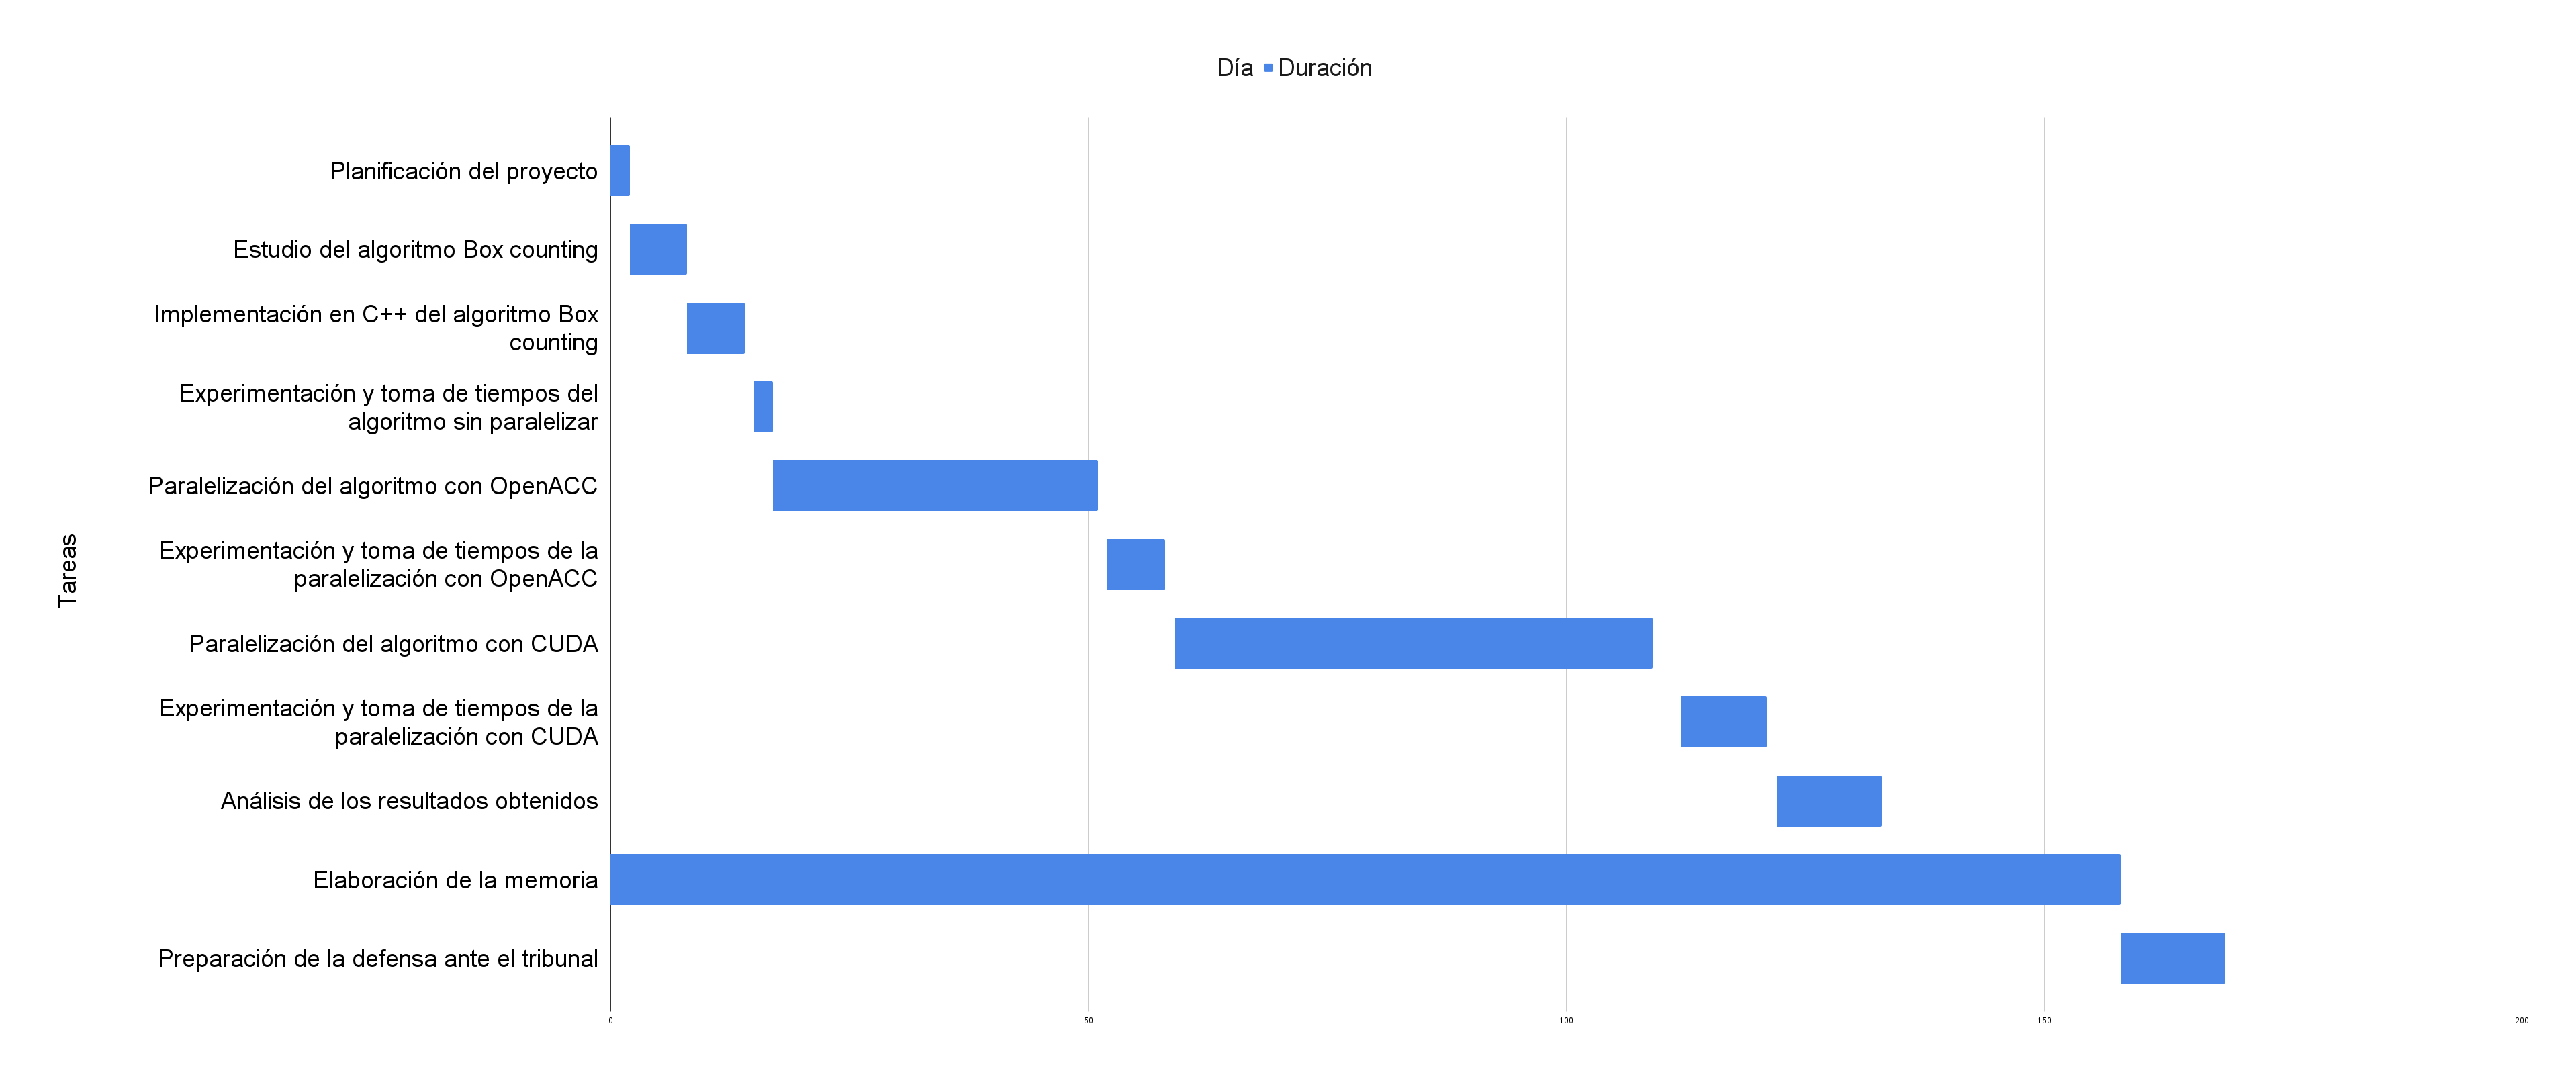
\includegraphics[scale=0.145]{img/Diagrama de Gantt2.png}
    \caption{Diagrama de Gantt}
    \label{fig:Gantt}
\end{figure}

\begin{table}[H]
    \centering
    \begin{adjustbox}{max height=\textheight, max width=\textwidth}
    \begin{tabular}{|clllrrl|} 
    \hline
    \rowcolor{black} \multicolumn{1}{|l}{}  & \textcolor{white}{Tareas} & \textcolor{white}{Fecha de inicio}         & \textcolor{white}{Fecha de finalización} & \textcolor{white}{Horas estimadas}&\\                                      
    \hline
    \rowcolor{white} \multicolumn{1}{|l}{}  & \textcolor{black}{Planificación del proyecto} & \textcolor{black}{1/2/2021}         & \textcolor{black}{3/2/2021} & \textcolor{black}{5}&\\
    \hline
    \rowcolor{white} \multicolumn{1}{|l}{}  & \textcolor{black}{Estudio del algoritmo Box counting} & \textcolor{black}{3/2/2021}         & \textcolor{black}{9/2/2021} & \textcolor{black}{10}&\\  
    \hline
    \rowcolor{white} \multicolumn{1}{|l}{}  & \textcolor{black}{Implementación en C++ del algoritmo Box counting} & \textcolor{black}{9/2/2021}         & \textcolor{black}{15/2/2021} & \textcolor{black}{10}\\
    \hline
    \rowcolor{white} \multicolumn{1}{|l}{}  & \textcolor{black}{Experimentación y toma de tiempos del algoritmo sin paralelizar} & \textcolor{black}{16/2/2021}         & \textcolor{black}{18/2/2021} &\textcolor{black}{5}&\\
    \hline
    \rowcolor{white} \multicolumn{1}{|l}{}  & \textcolor{black}{Paralelización del algoritmo con OpenACC} & \textcolor{black}{18/2/2021}         & \textcolor{black}{24/3/2021} &\textcolor{black}{70}\\
    \hline
    \rowcolor{white} \multicolumn{1}{|l}{}  & \textcolor{black}{Experimentación y toma de tiempos de la paralelización con OpenACC} & \textcolor{black}{25/3/2021}         & \textcolor{black}{31/3/2021} &\textcolor{black}{10}\\
    \hline
    \rowcolor{white} \multicolumn{1}{|l}{}  & \textcolor{black}{Paralelización del algoritmo con CUDA} & \textcolor{black}{1/4/2021}         & \textcolor{black}{21/5/2021} &\textcolor{black}{110}\\
    \hline
    \rowcolor{white} \multicolumn{1}{|l}{}  & \textcolor{black}{Experimentación y toma de tiempos de la paralelización con CUDA} & \textcolor{black}{24/5/2021}         & \textcolor{black}{2/6/2021} &\textcolor{black}{20}\\
    \hline
    \rowcolor{white} \multicolumn{1}{|l}{}  & \textcolor{black}{Análisis de los resultados obtenidos} & \textcolor{black}{3/6/2021}         & \textcolor{black}{14/6/2021} &\textcolor{black}{20}&\\
    \hline
    \rowcolor{white} \multicolumn{1}{|l}{}  & \textcolor{black}{Elaboración de la memoria} & \textcolor{black}{1/2/2021}         & \textcolor{black}{9/7/2021} &\textcolor{black}{30}&\\
    \hline
    \rowcolor{white} \multicolumn{1}{|l}{}  & \textcolor{black}{Preparación de la defensa ante el tribubal} & \textcolor{black}{9/7/2021}         & \textcolor{black}{20/7/2021} &\textcolor{black}{10}&\\                                  
    \hline
    \end{tabular}
    \end{adjustbox}
    \caption{Planificación temporal de las tareas}
    \label{fig:Planificacion}
\end{table}

\section{Recursos}
\subsection{Recursos Humanos}
Para la realización del proyecto se cuenta con Miguel Ángel Posadas Arráez como autor del mismo, y con el Profesor Dr. Juan Ruiz de Miras como tutor encargado de la supervisión del mismo.

\subsection{Recursos Software}
\label{RecursosSoftware}
Debido a que este proyecto corresponde al ámbito académico, se presta especial atención en utilizar herramientas con licencia libre, o que sean accesibles mediante la adquisición de algún tipo de licencia de estudiante, beneficiandonos así, de las ventajas que nos proporciona pertenecer a la Universidad de Granada.\\

\begin{itemize}
    \item Como alternativa a Matlab, se utiliza Octave. \cite{unknown-author-2021B}.
    \item Como herramienta de control de versiones, se utiliza GitHub, siendo posible obtener una licencia de estudiante en la siguiente referencia \cite{unknown-author-2021}.
    \item Para la elaboración de hojas de cálculo y generación de gráficos, se utiliza la suite ofimática de Google, accediendo siempre con la cuenta corporativa de la Universidad de Granada (dominio go.ugr.es).
    \item Para la elaboración de la memoria LaTeX como procesador de textos. \cite{unknown-author-no-dateD}.
    \item Para la paralelización mediante el uso de tarjeta gráfica, se utiliza el CUDA Toolkit, \cite{unknown-author-no-date}.
    \item Para la paralelización mediante el uso de los mútliples núcleos de la CPU, se utiliza OpenACC. \cite{unknown-author-no-dateB}.
    \item El sistema operativo del equipo principal utilizado para el desarrollo del proyecto es Ubuntu 20.04.2 LTS. \cite{unknown-author-no-dateE}.
\end{itemize}

\subsection{Recursos Hardware}
\label{RecursosHardware}
Para el desarrollo del proyecto se utilizan dos equipos, un ordenador portatil y un servidor. En la tabla \ref{fig:Hardware} quedan reflejadas las características más importantes de los distintos equipos.

\begin{table}[H]
    \centering
    \begin{adjustbox}{max height=\textheight,max width=\textwidth}
    \begin{tabular}{|clllrrl|} 
    \hline
    \rowcolor{black} \multicolumn{1}{|l}{}   & \textcolor{white}{Plataforma}         & \textcolor{white}{} \\  
    \hline
    \rowcolor{white} \multicolumn{1}{|l}{Plataforma}   & \textcolor{black}{PC}         & \textcolor{black}{Servidor} \\  
    \hline
    \rowcolor{white} \multicolumn{1}{|l}{Sistema Operativo}    & \textcolor{black}{Ubuntu 20.04 LTS $x86-64$}         & \textcolor{black}{Debian Linux 5.8.10-1 $x86-64$}        \\                                                            
    \hline
    \midrule
    \hline
    \rowcolor{black} \multicolumn{1}{|l}{}   & \textcolor{white}{CPU}         & \textcolor{white}{} \\  
    \hline
    \rowcolor{white} \multicolumn{1}{|l}{Model}    & \textcolor{black}{Intel(R) Core(TM) i7-7700HQ CPU @ 2.80GHz}         & \textcolor{black}{2 x Intel(R) Xeon(R) Silver 4210 CPU @ 2.20GHz}        \\ 
    \hline
    \rowcolor{white} \multicolumn{1}{|l}{Cores-thread}    & \textcolor{black}{4-8}         & \textcolor{black}{20-40}        \\  
    \hline
    \rowcolor{white} \multicolumn{1}{|l}{RAM}    & \textcolor{black}{12 GB}         & \textcolor{black}{96 GB}        \\ 
    \hline
    \rowcolor{black} \multicolumn{1}{|l}{}   & \textcolor{white}{GPU}         & \textcolor{white}{} \\  
    \hline                          
    \rowcolor{white} \multicolumn{1}{|l}{Model}    & \textcolor{black}{GeForce GTX 1050 Mobile}         & \textcolor{black}{GeForce RTX 3090}        \\ 
    \hline
    \rowcolor{white} \multicolumn{1}{|l}{Computing Capability}   & \textcolor{black}{6.1}         & \textcolor{black}{8.0} \\  
    \hline
    \rowcolor{white} \multicolumn{1}{|l}{Arquitectura}   & \textcolor{black}{Pascal}         & \textcolor{black}{Ampere} \\  
    \hline 
    \rowcolor{white} \multicolumn{1}{|l}{MPs}   & \textcolor{black}{5}         & \textcolor{black}{82} \\  
    \hline 
    \rowcolor{white} \multicolumn{1}{|l}{SPs}   & \textcolor{black}{640}         & \textcolor{black}{10496} \\  
    \hline  
    \rowcolor{white} \multicolumn{1}{|l}{Memoria Global}   & \textcolor{black}{2 GB}         & \textcolor{black}{24 GB} \\  
    \hline  
    \rowcolor{white} \multicolumn{1}{|l}{Tamaño de Warp}   & \textcolor{black}{32}         & \textcolor{black}{32} \\  
    \hline  
    \rowcolor{white} \multicolumn{1}{|l}{Nº Máximo de hebras por bloque}   & \textcolor{black}{1024}         & \textcolor{black}{1024} \\  
    \hline  
    \rowcolor{white} \multicolumn{1}{|l}{Nº Máximo de hebras por SMP}   & \textcolor{black}{2048}         & \textcolor{black}{1536} \\  
    \hline  
    \rowcolor{white} \multicolumn{1}{|l}{Tamaño de caché L2}   & \textcolor{black}{524288 B}         & \textcolor{black}{6291456 B} \\  
    \hline  
    \rowcolor{white} \multicolumn{1}{|l}{Memoria compartida por bloque}   & \textcolor{black}{49152 B}         & \textcolor{black}{49152 B} \\  
    \hline  
    \rowcolor{white} \multicolumn{1}{|l}{Registros por bloque}   & \textcolor{black}{65536}         & \textcolor{black}{65536} \\  
    \hline  
    \rowcolor{white} \multicolumn{1}{|l}{ECC}   & \textcolor{black}{Desactivado}         & \textcolor{black}{Desactivado} \\  
    \hline  
    \rowcolor{white} \multicolumn{1}{|l}{Consumo energético}   & \textcolor{black}{75 W}         & \textcolor{black}{350 W} \\  
    \hline    
    \end{tabular}
    \end{adjustbox}
    \caption{Tabla comparativa de las plataformas hardware y software utilizadas para las medidas de tiempos}
    \label{fig:Hardware}
\end{table}



El primer equipo (Identificado como PC en la Tabla \ref{fig:Hardware}) tuvo un coste inicial de 1100€, basándonos en \cite{unknown-author-no-dateG}, tiene un periodo de amortización de 6 años, luego cada año tiene un coste de 183.33€. Como este proyecto está enmarcado en un cuatrimestre, se estima que el coste de amortización del equipo es de 45.83€.\\

El servidor tiene un precio de 24000€, se establece un periodo de amortización de 6 años basándonos de nuevo en \cite{unknown-author-no-dateG}. Obtenemos que el del servidor tiene un costo de 4000€/año, que resulta en 11€/día. Como se han requerido 7 días del servidor, concluimos que el costo total por este recurso ha sido de 77€.\\ 

\subsection{Organización del personal}
Dentro del plan de estudios de la titulación \cite{unknown-author-no-dateC}, el Trabajo de Fin de Grado (TFG), tiene una carga de 12 créditos ECTS. Sabiendo que cada crédito ECTS equivale a 25 horas, el proyecto debe ser planificado en un total de 300 horas.\\


\subsection{Estimación de costos del proyecto}
\label{Costos}

Como ya se ha comentado previamente, el proyecto debe ser planificado en 300 horas, por tanto en este apartado se va a realizar un desglose de los gastos que conlleva el proyecto, especificando a que se dedicará cada hora. Para el cálculo del presupuesto se va a tomar como salario promedio 8.22 €/hora según lo especificado en \cite{unknown-author-2021C}.\\ En la Tabla \ref{fig:CosteTareas} se puede consultar el desglose de los gastos de cada tarea.

\begin{table}[H]
    \centering
    \begin{adjustbox}{max height=\textheight,max width=\textwidth}
    \begin{tabular}{|clllrrl|} 
    \hline
    \rowcolor{black} \multicolumn{1}{|l}{}  & \textcolor{white}{Tareas} & \textcolor{white}{Duración (h)}         & \textcolor{white}{Importe (€)} \\                                      
    \hline
    \rowcolor{white} \multicolumn{1}{|l}{}  & \textcolor{black}{Planificación del proyecto} & \textcolor{black}{5 h}         & \textcolor{black}{41.1€} &\\
    \hline
    \rowcolor{white} \multicolumn{1}{|l}{}  & \textcolor{black}{Estudio del algoritmo Box counting} & \textcolor{black}{10 h}         & \textcolor{black}{82.2€} &\\  
    \hline
    \rowcolor{white} \multicolumn{1}{|l}{}  & \textcolor{black}{Implementación en C++ del algoritmo Box counting} & \textcolor{black}{10 h}         & \textcolor{black}{82.2€} \\
    \hline
    \rowcolor{white} \multicolumn{1}{|l}{}  & \textcolor{black}{Experimentación y toma de tiempos del algoritmo sin paralelizar} & \textcolor{black}{5 h}         & \textcolor{black}{41.1€}&\\
    \hline
    \rowcolor{white} \multicolumn{1}{|l}{}  & \textcolor{black}{Paralelización del algoritmo con OpenACC} & \textcolor{black}{70 h}         & \textcolor{black}{575.4€} &\\
    \hline
    \rowcolor{white} \multicolumn{1}{|l}{}  & \textcolor{black}{Experimentación y toma de tiempos de la paralelización con OpenACC} & \textcolor{black}{10 h}         & \textcolor{black}{82.2€} &\\
    \hline
    \rowcolor{white} \multicolumn{1}{|l}{}  & \textcolor{black}{Paralelización del algoritmo con CUDA} & \textcolor{black}{110 h}         & \textcolor{black}{904.2€} \\
    \hline
    \rowcolor{white} \multicolumn{1}{|l}{}  & \textcolor{black}{Experimentación y toma de tiempos de la paralelización con CUDA} & \textcolor{black}{20 h}         & \textcolor{black}{164.4€} &\\
    \hline
    \rowcolor{white} \multicolumn{1}{|l}{}  & \textcolor{black}{Análisis de los resultados obtenidos} & \textcolor{black}{20 h}         & \textcolor{black}{164.4€} &\\
    \hline
    \rowcolor{white} \multicolumn{1}{|l}{}  & \textcolor{black}{Elaboración de la memoria} & \textcolor{black}{30 h}  &\textcolor{black}{246.6€}&\\
    \hline
    \rowcolor{white} \multicolumn{1}{|l}{}  & \textcolor{black}{Preparación de la defensa ante el tribubal} & \textcolor{black}{10 h}         & \textcolor{black}{82.2€} &\\                                  
    \hline
    \rowcolor{white} \multicolumn{1}{|l}{}  & \textcolor{black}{Total} & \textcolor{black}{300h}         & \textcolor{black}{2466€} &\\                                  
    \hline
    \end{tabular}
    \end{adjustbox}
    \caption{Desglose de costes de las tareas}
    \label{fig:CosteTareas}
\end{table}

En la Tabla \ref{fig:CosteRecursos} se especifican todos los recursos necesarios para la realización del proyecto con su coste asociado.

\begin{table}[H]
    \centering
    \begin{adjustbox}{max height=\textheight, max width=\textwidth}
    \begin{tabular}{|clllrrl|} 
    \hline
    \rowcolor{black} \multicolumn{1}{|l}{}  & \textcolor{white}{Recursos} & \textcolor{white}{Importe (€)}         & \textcolor{white}{Detalle} \\                                      
    \hline
    \rowcolor{white} \multicolumn{1}{|l}{}  & \textcolor{black}{Recursos Humanos} & \textcolor{black}{2466€ €}         & \textcolor{black}{Total obtenido en la Tabla \ref{fig:CosteTareas}} &\\
    \hline
    \rowcolor{white} \multicolumn{1}{|l}{}  & \textcolor{black}{Conexión a Internet} & \textcolor{black}{90 €}         & \textcolor{black}{6 meses desde febrero hasta julio a un precio de 15€/mes } &\\
    \hline
    \rowcolor{white} \multicolumn{1}{|l}{}  & \textcolor{black}{Recursos Software} & \textcolor{black}{0 €}         & \textcolor{black}{Ver \textit{\nameref{RecursosSoftware}}} &\\
    \hline
    \rowcolor{white} \multicolumn{1}{|l}{}  & \textcolor{black}{Amortización del equipo personal} & \textcolor{black}{45.83 €}         & \textcolor{black}{Coste de amortización del equipo detallado en \textit{\nameref{RecursosHardware}}} &\\
    \hline
    \rowcolor{white} \multicolumn{1}{|l}{}  & \textcolor{black}{Amortización del servidor} & \textcolor{black}{77 €}         & \textcolor{black}{Coste de amortización del servidor detallado en \textit{\nameref{RecursosHardware}}} &\\
    \hline
    \rowcolor{white} \multicolumn{1}{|l}{}  & \textcolor{black}{Total} & \textcolor{black}{2678.83 €}         & \textcolor{black}{} &\\
    \hline
    \end{tabular}
    \end{adjustbox}
    \caption{Desglose de costes de los recursos}
    \label{fig:CosteRecursos}
\end{table}

	
	\chapter{El algoritmo}

El cálculo de la dimensión fractal de una estructura de datos proporciona información relevante sobre la propia estructura, ya que el análisis fractal analiza su estructura geométrica a múltiples niveles.\\

El método utilizado en este proyecto se llama Box counting. Su funcionamiento reside en la subdivisión de la estructura de datos en cajas, con el objetivo de poder analizar la estructura en una escala más pequeña. El nombre de Box counting viene dado ya que el algoritmo, en esencia, lo que hace es contar la cantidad de cajas (de distintos tamaños) que hay en la estructura. Por esto mismo, antes decíamos que el análisis fractal analiza la estructura a múltiples niveles, porque el algoritmo empieza contando cajas de la menor dimensión posible (1) y acaba por contar las cajas de mayor tamaño posible (el de la estructura de datos).\\

Cuando aplicamos el algoritmo Box counting, nos interesa el cálculo de dos medidas:


\begin{itemize}
    \item \textbf{N}: Representa el número de cajas \textit{válidas} que hay presentes en la estructura.
    \item \textbf{r}: Representa el tamaño de las cajas. 
\end{itemize}
 
Como ya se ha comentado antes, el algoritmo realiza un análisis multinivel de la estructura, es decir que no solo obtenemos un valor de N y otro de r, si no que para cada valor de r (es decir, para cada tamaño de la caja) obtenemos un valor de N (una cantidad de cajas de tamaño r). El cálculo de la dimensión fractal (D) viene dado por la siguiente expresión \ref{formula}.

En las Figuras \ref{fig:basico1} y \ref{fig:basico2} , se aprecia el análisis multinivel del que hablamos. En función del tamaño de la caja el número de cajas válidas cambia.

\begin{equation}
    \label{formula}
    D = \frac{log(N)}{log(r)}
\end{equation}

\begin{figure}[H]
    \centering
    
\includegraphics[width=.24\textwidth]{img/basico1.png}
    
\includegraphics[width=.24\textwidth]{img/basico2.png}
    \caption{Simplificación algoritmo con r = 1 (Izquierda) y r = 2 (Derecha)}
    \label{fig:basico1}
\end{figure}

\begin{figure}[H]
    \centering
    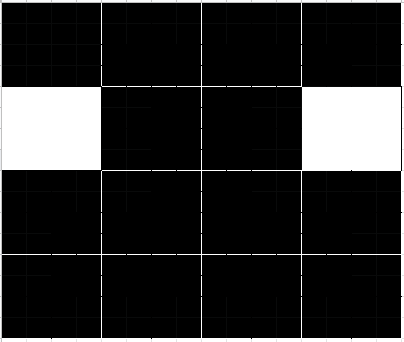
\includegraphics[width=.24\textwidth]{img/basico3.png}
    
\includegraphics[width=.24\textwidth]{img/basico4.png}
    \caption{Simplificación algoritmo con r = 4 (Izquierda) y r = 8 (Derecha)}
    \label{fig:basico2}
\end{figure}



\section{Aplicación del método Box counting para el cálculo de la dimensión fractal de matrices binarias}

El algoritmo sobre el que se sustenta este proyecto tiene 3 características destacables:

\begin{itemize}
    \item \textbf{Método de escaneo}: Se trata de la manera que tenémos de recorrer la matriz, en el algoritmo utilizado para este proyecto se utiliza un método de escaneo de cuadrícula fija ( \textit{"fixed grid scans"} en inglés) \cite{unknown-author-no-dateF}. Esto quiere decir que a la hora de subdividir la estructura de datos en cajas, se hará de manera que para cada tamaño de caja seleccionado, un elemento de la matriz pertenecerá únicamente a una caja, sin que exista la posibilidad de que un elemento este en dos cajas para una misma subdivisión.
    \item \textbf{Criterio de validez}: Una vez tengamos la estructura de datos divididas en cajas del mismo tamaño, tenemos que establecer una regla para decidir sin contar la caja como válida o no. En este caso es necesario hacer una distinción:
    \begin{itemize}
        \item Sí  r = 1 , se cuenta el elemento como válido siempre que el elemento valga 1.
        \item Sí  r > 1 , se realiza una operación OR con todos los elementos de la caja. En caso de que el resultado de la operación sea 1 se contará la caja como válida. 
    \end{itemize}
    \item \textbf{Aumento del tamaño de la caja}: En cada iteración el tamaño de la caja aumenta siguiendo las potencias de 2 (1,2,4...) hasta llegar al tamaño de las dimensiones de la matriz. Se trabaja con matrices cuadradas con tamaños de fila o columna potencia de 2.
\end{itemize}


Como se adelanta en la última característica comentada, el cálculo de r no supone ninguna complicación, ya que conociendo el tamaño de la matriz cuadrada, simplemente consiste en crear una lista cuyos valores sean las potencias de 2 hasta el tamaño de la matriz.\\

Sin embargo, el cálculo de las cajas que cumplen el criterio de validez, es más complejo y requiere de un coste computacional bastante más elevado. En el Listado \ref{MatBox2D}, que corresponde a la implementación en Matlab de la que se parte como base para el proyecto \cite{unknown-author-2008}, se aprecia la aplicación del algoritmo para el cálculo de N (número de cajas válidas).\\

\begin{lstlisting}[language=Matlab,caption={Código Matlab del método Box counting para matrices bidimensionales. Las variables de entrada del código son la matriz c (matriz binaria que queremos analizar), la lista n (inicialmente vacía, contendrá el número de cajas válidas para cada tamaño de caja) y la variable p. que representa el número de iteraciones necesarias para cubrir la matriz entera, teniendo en cuenta que cada iteración aumenta el tamaño de la caja en una potencia de dos.},label=MatBox2D]
n(p+1) = sum(c(:));
for g=(p-1):-1:0
    $\Comment{//siz es el valor de r, es decir el tamaño de la caja}$
    siz = 2^(p-g);
    $\Comment{//siz2 es utilizada para localizar el resultado de }$
    $\Comment{//la operación OR del r de la anterior iteración. }$
    $\Comment{//Las casillas roja en las figuras de la sección 3.3 }$
    siz2 = round(siz/2);
    $\Comment{//Estos bucles son los encargados de realizar el cálculo del OR}$
    for i=1:siz:(width-siz+1)
        for j=1:siz:(width-siz+1)
            c(i,j) = ( c(i,j) || c(i+siz2,j) || ...
                                c(i,j+siz2) || c(i+siz2,j+siz2) );
        end
    end
    $\Comment{//Se acumula el número de 1 (se calcula el N para el r dado)}$
    n(g+1) = sum(sum(c(1:siz:(width-siz+1),1:siz:(width-siz+1))));
end
\end{lstlisting}

\section{Orden del algoritmo}
\label{Orden}
Para realizar un estudio del orden del algoritmo del Listado \ref{MatBox2D}, debemos diferenciar entre los bucles internos y el bucle  externo.\\

Los bucles internos, en el peor de los casos, tienen que recorrer la estructura de datos al completo (en dos ocasiones, líneas 10-15 y línea 17 en Listado \ref{MatBox2D}). Por tanto, la expresión \ref{eficiencia_interna} (donde el 2 representa las dos operaciones elementales previas, el cálculo de la variable siz y siz2) caracteriza el tiempo de ejecución del interior del bucle externo, es decir, el contenido de las líneas 3 - 17 . Como la notación O trata de acotar superiormente, podemos concluir que dicha parte del algoritmo tiene un orden de O($n^2$).\\

\begin{equation}
    \label{eficiencia_interna}
    n^2 + n^2 + 2 = 0
\end{equation}

Por otro lado, el bucle externo realiza un total de p iteraciones, siendo p el $log_2(n)$. Por tanto, la expresión \ref{eficiencia} caracteriza el tiempo de ejecución del código del Listado \ref{MatBox2D}, siendo acotada superiormente por $log_2(n)*n^2$, por lo que podemos decir que el código es de orden O( $log_2(n)*n^2$). 

\begin{equation}
    \label{eficiencia}
    log_2(n)*(n^2 + n^2 + 2) = 0
\end{equation}

Se recuerda que en este proyecto no se ha trabajado únicamente con matrices bidimensionales, si no que también se ha trabajado con matrices tridimensionales y cuatridimensionales. Conforme aumenta la complejidad de la estructura de datos, aumenta la complejidad para recorrerla, siendo el algoritmo de orden O($log_2(n)*n^3$) para matrices con tres dimensiones y O($log_2(n)*n^4$) para matrices con cuatro dimensiones.
\section{Ejemplo para una matriz bidimensional}
Con el objetivo de clarificar el funcionamiento del algoritmo se dejan las Figuras \ref{fig:alg1}, \ref{fig:alg2} y \ref{fig:alg3}, con la representación del funcionamiento del algoritmo para una matriz bidimensional de 16x16.

\begin{figure}[H]
    \centering
    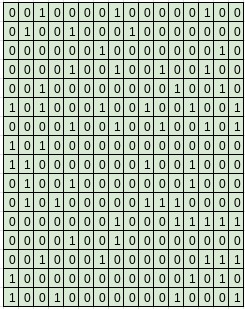
\includegraphics[width=.24\textwidth]{img/ejemploAlgoritmo1.jpeg}
    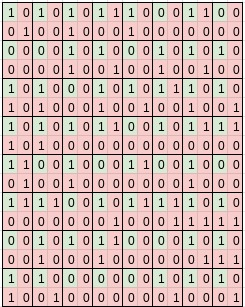
\includegraphics[width=.24\textwidth]{img/ejemploAlgoritmo2.jpeg}
    \caption{Iteraciones con r = 1 (Izquierda) y r = 2 (Derecha)}
    \label{fig:alg1}
\end{figure}

\begin{figure}[H]
    \centering
    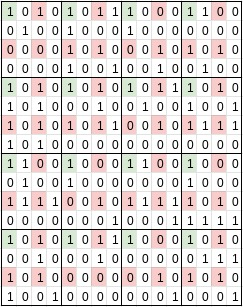
\includegraphics[width=.24\textwidth]{img/ejemploAlgoritmo3.jpeg}
    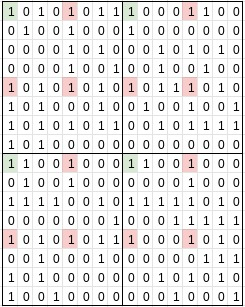
\includegraphics[width=.24\textwidth]{img/ejemploAlgoritmo4.jpeg}
    \caption{Iteraciones con r = 4 (Izquierda) y r = 8 (Derecha)}
    \label{fig:alg2}
\end{figure}

\begin{figure}[H]
    \centering
    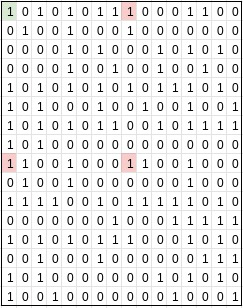
\includegraphics[width=.24\textwidth]{img/ejemploAlgoritmo5.jpeg}
    \caption{Iteracion con r = 16}
    \label{fig:alg3}
\end{figure}


Las casillas señaladas con el color verde corresponden a las casillas que son contadas a la hora de calcular el N (línea 16 en Listado \ref{MatBox2D}). Para el cálculo del valor de las casillas de color verde, se hace una operación OR con los valores calculados en la iteración anterior, es decir la casilla verde y las tres casillas señaladas de color rojo en las Figuras \ref{fig:alg1}, \ref{fig:alg2} y \ref{fig:alg3} (ver líneas 9-15 en Listado \ref{MatBox2D}).

	\chapter{Tecnologías utilizadas}
Tras el estudio teórico del algoritmo a implementar, se deja este capítulo para la introducción y descripción de las tecnologías a utilizar durante el proyecto. El uso de estas tecnologías tiene como objetivo explotar el paralelismo que proporcionan los recursos de los equipos detallados en la sección \ref{RecursosHardware}.

\section{El estándar de programación OpenACC}
\label{OpenACC}
OpenACC.org \cite{unknown-author-no-dateB} es una organización sin ánimo de lucro que cuenta con grandes empresas como Nvidia, AMD o Cray como miembros. El objetivo de esta organización es proporcionar el estándar de programación OpenACC.

OpenACC ofrece a los desarrolladores una API soportada por C/C++ y Fortran, compatible con mútliples plataformas hardware. Siendo posible el uso de esta API tanto en procesadores Intel como AMD, incluso en tarjetas gráficas de Nvidia (aunque en este proyecto únicamente se utilizará para explotar el paralelismo a nivel de procesador).

El funcionamiento de OpenACC consiste en definir mediante la API comentada anteriormente, los bucles o zonas del código en los que existe cierto nivel de paralelismo (esto es tarea del programador) y el compilador se encarga de añadir todas las operaciones necesarias para acelerar la región definida utilizando los distintos núcleos del procesador.

Existen mútliples compiladores que soportan este estándar de programación, para este proyecto se ha utilizado pgc++ que viene incluido en el Nvidia HPC SDK \cite{unknown-author-2021D}.

Para este proyecto se ha utilizado la siguiente especificación de OpenACC \cite{unknown-author-2019}.


\section{La plataforma de programación paralela CUDA}

CUDA, \textit{(Compute Unified Device Architecture)} es una plataforma de programación paralela desarrollada por Nvidia. Permite al programador aprovechar la computación de propósito general en unidades de procesamiento gráfico (GPGPU) para acelerar el código desarrollado. \cite{unknown-author-2021E}.

Puede ser utilizado junto a varios lenguajes de programación distintos, pero el lenguaje de programación utilizado para el desarrollo de los kernels de CUDA es C (En CUDA, un kernel es una función que será ejecutada por tantas \textit{threads} como lancemos).

Para el uso de CUDA, Nvidia nos proporciona lo que se conoce como CUDA Toolkit. Se trata de un kit que incorpora una serie de herramientas que ayudan al desarrollador en la tarea del desarrollo. Algunas de estas herramientas son:

\begin{itemize}
    \item CUDA NVCC: El compilador utilizado para los archivos con extensión .cu (archivos CUDA).
    \item Una serie de librerías muy utilizadas en la programación CUDA, como lo son cudart, cuRAND, cuSOLVER, cuSPARSE \dots
    \item CUDA GDB: Un depurador compatible con programas CUDA.
    \item CUDA Memcheck: Una herramienta que es capaz de detectar errores de memoria como accesos a posiciones fuera de los límites en programas CUDA
    \item cuobjdump: Permite obtener información sobre los archivos binarios resultado de la compilación con NVCC.
    \item nvprof: Una herramienta de profiling que permite realizar una monitorización del ejecutable para conocer en que zonas del código se está consumiendo más tiempo.
    \item pgc++: El compilador utilizado para OpenACC que hemos comentado en la sección \ref{OpenACC}.
\end{itemize}

Para el desarrollo de éste proyecto se ha utilizado la versión 11.2 del CUDA Toolkit \cite{unknown-author-2021F}.

\section{OpenACC vs CUDA}

Una vez introducidas las tecnologías que van a ser utilizadas en este proyecto se deja esta sección a modo de comparativa entre OpenACC y CUDA.

OpenACC es una tecnología sencilla de utilizar, ya que sobre el código secuencial escrito en C++ se añaden las directivas necesarias para explotar el paralelismo a nivel de bucle. Esto quiere decir, que no es necesaria utilizar una metodología para la programación distinta a la que se ha utilizado para el código secuencial.

CUDA es una tecnología algo más compleja, ya que si requiere el estudio de conceptos como lo son los kernels, blocks, threads, grid \dots Además, requiere cambiar el código secuencial inicial para utilizar la API de CUDA para operaciones como la reserva de memoria. Por otro lado, no es posible el uso de los vectores de la STL utilizados en la versión secuencial, sino que es necesaria la gestión de la memoria a través de punteros. Finalmente, por limitaciones de CUDA, no es posible la gestión de arrays multinivel sin el uso de librerías externas, por lo que es necesaria la linealización de las estructuras de datos.

Pese a que CUDA presente más complejidad, los beneficios que nos proporciona el uso del paradigma GPGPU son sustancialmente superiores a los que nos proporciona OpenACC. Aunque es necesario recalcar que CUDA requiere la transferencia de las estructuras de datos a la tarjeta gráfica, por lo que la estructura de datos a analizar debe tener un tamaño considerable para que el tiempo de la transferencia a la tarjeta gráfica se contrareste con los beneficios computacionales que nos proporciona la GPU.

	\chapter{Implementación secuencial en C++}
\label{Secuencial}
Antes de utilizar las tecnologías introducidas en el Capítulo \ref{Tecnologias}, es necesario realizar una implementación en un lenguaje que permita el uso de dichas tecnologías. Para este proyecto se realiza una implementación en C++, y se modelan las estructuras de datos con vectores de la STL \cite{unknown-author-no-dateH}.

Para esta implementación, se parte de un código inicial, \cite{unknown-author-2008}, modificado por el tutor del proyecto, el Profesor D. Juan Ruiz de Miras, para que el algoritmo sea capaz de analizar matrices en 4 dimensiones.



En primer lugar se parte de la versión bidimensional, ya que es más sencilla y es más fácil detectar errores. La versión bidimensional en Matlab es la que se puede consultar en el Listado \ref{MatBox2D}. El equivalente programado en C++ se describe en el Listado \ref{CppBox2D}. Como variables de entrada en el código está \textbf{p} que representa el número de iteraciones necesarias para cubrir la matriz. \textbf{matriz} que es la estructura de datos y \textbf{n} que es la lista en la que se almacenará la cantidad de cajas válidas para cada tamaño de caja.
\newpage
\begin{lstlisting}[language=C++,caption={Primera versión del Boxcount2D programado en C++},label=CppBox2D]
for(auto g=p; g >= 0; g--)
{
    int siz = pow(2,(p-g));
    int siz2 = round(siz/2);
    for(auto i = 0; i <= (width-siz); i += siz)
        for(auto j = 0; j <= (width-siz); j += siz)
            matriz[i][j] = (matriz[i][j] 
                            || matriz[i+siz2][j] 
                            || matriz[i][j+siz2] 
                            || matriz[i+siz2][j+siz2]);

    int suma = 0; 
    for(auto i = 0; i <= (width-siz); i += siz)
        for(auto j = 0; j <= (width-siz); j += siz)
            suma += matriz[i][j];

    n.push_back(suma);
}
\end{lstlisting}

\newpage

Como se anticipaba en la sección \ref{Orden}, la implementación de las versiones para matrices tridimensionales y cuatridimensionales son muy similares a la versión bidimensional, aunque aumentando la complejidad de la indexación de la estructura de datos. En el Listado \ref{CppBox3D} y \ref{CppBox4D} se aprecia dicho aumento de complejidad.

\begin{lstlisting}[language=C++,caption={Primera versión del Boxcount3D programado en C++},label=CppBox3D]
for(auto g=p; g >= 0; g--)
{
    int siz = pow(2,(p-g));
    int siz2 = round(siz/2);
    for(auto i = 0; i <= (width-siz); i += siz)
        for(auto j = 0; j <= (width-siz); j += siz)
            for(auto k = 0; k <= (width-siz); k += siz)
                matriz[i][j][k] = (    matriz[i][j][k] 
                                || matriz[i+siz2][j][k] 
                                || matriz[i][j+siz2][k] 
                                || matriz[i+siz2][j+siz2][k] 
                                || matriz[i][j][k+siz2] 
                                || matriz[i+siz2][j][k+siz2] 
                                || matriz[i][j+siz2][k+siz2] 
                        || matriz[i+siz2][j+siz2][k+siz2]);

    int suma = 0; 
    for(auto i = 0; i <= (width-siz); i += siz)
        for(auto j = 0; j <= (width-siz); j += siz)
            for(auto k = 0; k <= (width-siz); k += siz)
                suma += matriz[i][j][k];

    n.push_back(suma);
}
\end{lstlisting}

\newpage
\begin{lstlisting}[language=C++,caption={Primera versión del Boxcount4D programado en C++},label=CppBox4D,basicstyle=\tiny]
for(auto g=p; g >= 0; g--)
{
    int siz = pow(2,(p-g));
    int siz2 = round(siz/2);
    for(auto i = 0; i <= (width-siz); i += siz)
        for(auto j = 0; j <= (width-siz); j += siz)
            for(auto k = 0; k <= (width-siz); k += siz)
                for(auto l = 0; l <= (width-siz); l += siz)
                    matriz[i][j][k][l] = (  matriz[i][j][k][l] 
                                            || matriz[i+siz2][j][k][l] 
                                            || matriz[i][j+siz2][k][l] 
                                            || matriz[i+siz2][j+siz2][k][l] 
                                            || matriz[i][j][k+siz2][l] 
                                            || matriz[i+siz2][j][k+siz2][l] 
                                            || matriz[i][j+siz2][k+siz2][l] 
                                            || matriz[i+siz2][j+siz2][k+siz2][l] 
                                            || matriz[i][j][k][l+siz2] 
                                            || matriz[i+siz2][j][k][l+siz2] 
                                            || matriz[i][j+siz2][k][l+siz2] 
                                            || matriz[i+siz2][j+siz2][k][l+siz2] 
                                            || matriz[i][j][k+siz2][l+siz2] 
                                            || matriz[i+siz2][j][k+siz2][l+siz2] 
                                            || matriz[i][j+siz2][k+siz2][l+siz2] 
                                            || matriz[i+siz2][j+siz2][k+siz2][l+siz2] );

    int suma = 0; 
    for(auto i = 0; i <= (width-siz); i += siz)
        for(auto j = 0; j <= (width-siz); j += siz)
            for(auto k = 0; k <= (width-siz); k += siz)
                for(auto l = 0; l <= (width-siz); l += siz)
                    suma += matriz[i][j][k][l];

    n.push_back(suma);
}
\end{lstlisting}

Es necesario destacar que estas versiones no son las finales, son las que se utilizan como base para la implantación de las diferentes tecnologías. A lo largo de los siguientes capítulos se exponen diversas modificaciones que se realizan para optimizar el código, estas modificaciones también se aplican a la versión secuencial para que las comparaciones se hagan en igualdad de condiciones.

Una vez implementada la versión secuencial, es importante saber en qué zonas del código se consume más tiempo de ejecución. Para esto se ha utilizado una herramienta de profiling llamada \textit{gprof}, \cite{unknown-author-no-dateI}. Con esta herramienta se confirma lo que se sospechaba, la mayor parte del tiempo el código se ocupa en labores de gestión de memoria, tanto en el acceso mediante el operador [], como en la escritura del resultado de las operaciones OR. Esto es un factor a tener en cuenta ya que esas son las zonas que tenemos que paralelizar. Los resultados de esta herramienta eran de esperar ya que las operaciones de Entrada/Salida son muy costosas.

	\chapter{Paralelización con OpenACC}
\label{ParalelizacionOpenACC}
En este capítulo se va a describir la paralelización realizada con la tecnología OpenACC introducida en la Sección \ref{OpenACC}, sobre el código secuencial desarrollado en el Capítulo \ref{Secuencial}.

Si analizamos el Listado \ref{CppBox2D}, vemos que hay dos zonas de las que se puede aprovechar el paralelismo. La primera zona es la que corresponde a las líneas 5-8, ya que distintas hebras pueden realizar el cómputo del box simultáneamente, sin interferirse entre ellas, ya que estamos usando el \textit{"fixed grid scans"}, es decir, que cada elemento de la matriz únicamente pertenece un a box. Para paralelizar esta parte con OpenACC es necesario utilizar las directivas necesarias para que las distintas hebras hebras se repartan las iteraciones de los bucles. Esta directiva es \textit{parallel loop} 

La segunda zona en la que se puede extraer paralelismo, es en la zona en la que se acumulan la cantidad de cajas válidas, es decir, en las líneas 10-13. Pero es necesario apreciar un detalle, todas las hebras que se lancen van a actualizar la misma variable \textit{suma}, por lo que aparece lo que se conoce como \textbf{condición de carrera}. No todas las hebras finalizan su ejecución al mismo tiempo, y esto puede ocasionar que la variable \textit{suma} acabe con un resultado erróneo. Para solventar esta problemática, es necesario que establezcamos los mecanismos necesarios para que el acceso a la variable \textit{suma} (sección crítica) se realice bajo la condición de \textbf{exclusión mútua}. Por tanto para paralelizar esta zona con OpenACC será necesario no sólo las directivas necesarias para que se repartan las iteraciones de los bucles entre las distintas hebras, si no establecer las directivas necesarias para que el cálculo de la variable \textit{suma} se haga correctamente.

En el Listado \ref{ACCBox2D} se puede consultar la primera versión del Boxcount2D utilizando OpenACC. Finalmente, para solucionar el problema que sufre el cálculo de la variable \textit{suma}, se opta por la utilización de la cláusula \textit{reduce} que permite a cada hebra almacenar una copia privada de su variable \textit{suma}, para finalmente obtener el variable real mediante la acumulación de las variables privadas de cada hebra.


\begin{lstlisting}[language=C++,caption={Primera versión del Boxcount2D paralelizado con OpenACC},label=ACCBox2D]
    for(auto g=p; g >= 0; g--)
    {
        int siz = pow(2,(p-g));
        int siz2 = round(siz/2);
        #pragma acc parallel loop 
        for(auto i = 0; i <= (width-siz); i += siz)
            for(auto j = 0; j <= (width-siz); j += siz)
                matriz[i][j] = (    matriz[i][j] 
                                ||  matriz[i+siz2][j] 
                                ||  matriz[i][j+siz2] 
                                ||  matriz[i+siz2][j+siz2]);
    
        int suma = 0; 
        #pragma acc parallel loop independent reduction(+:suma)
        for(auto i = 0; i <= (width-siz); i += siz)
            for(auto j = 0; j <= (width-siz); j += siz)
                suma += matriz[i][j];
    
        n.push_back(suma);
    }
\end{lstlisting}

Aunque la complejidad en el orden de los algoritmos para la versión 3D y 4D sea superior, la paralelización con OpenACC es idéntica para las versiones tridimensionales y cuatridimensionales, requeriendo estas del uso de las mismas directivas.

	\chapter{Paralelización con CUDA}
\label{ParalelizacionCUDA}

En este capítulo se va a describir la paralelización realizada con la plataforma de programación CUDA, introducida en la sección \ref{CUDA}. Como se anticipaba en la comparativa de la sección \ref{comparativa}, CUDA es, objetivamente, una tecnología más compleja, ya que para aplicarla es necesario estudiar una serie de conceptos como \textit{kernel, thread, block, grid, thread per block \dots }. 

\section{Funcionamiento de CUDA}
\label{FuncionamientoCUDA}
Para la implementación de una versión con CUDA, es necesario saber el funcionamiento de esta plataforma de programación. En primer lugar, debemos reservar memoria principal para el almacenamiento de la estructura de datos que se va a procesar. Una vez tengamos la estructura de datos correctamente alojada en memoria, es el momento de la transferencia CPU-GPU, es decir, se transfiere la estructura de datos a la tarjeta gráfica. La transferencia de la estructura de datos es un proceso costoso, y es el \textit{precio a pagar} por utilizar la programación GPU. Por tanto, tenemos que asegurarnos que las dimensiones de la estructura de datos son suficientemente grandes para que sea rentable consumir ese tiempo en la transferencia, ya que si la estructura de datos es de un tamaño considerable aunque se consuma tiempo de transferencia de datos, este se verá compensando por la aceleración que proporciona el uso de la arquitectura SIMD (\textit{"Single Instruction Multiple Data"}) en este tipo de operaciones.

Una vez tengamos la estructura de datos en la tarjeta gráfica es el momento de procesarla. Tendremos que programar un \textit{kernel}, podemos ver un \textit{kernel} de CUDA como una función ejecutada en la tarjeta gráfica. Se lanzarán tantos \textit{kernels} como \textit{threads} hayamos lanzado. Las \textit{threads} se lanzarán por grupos, estos grupos son llamados \textit{blocks} y a su vez estos \textit{blocks} pueden ser lanzados en grupos llamados \textit{grids}.

Como ya hemos comentado, las \textit{threads} se lanzan por grupos llamados \textit{blocks}, de aquí aparece un nuevo concepto, el llamado \textit{thread per block}, es decir, el número de \textit{threads} que hay en cada \textit{block}, queda como tarea del programador establecer este parámetro. Es importante saber que las tarjetas gráficas de Nvidia cuentan con \textit{warps} (unidades de ejecución) de 32 \textit{threads} ver \cite{unknown-author-2021G}, por tanto por motivos de eficiencia se tomarán valores de \textit{thread per block} mútliplos de 32, teniendo como límite en las tarjetas gráficas actuales 1024. 

\section{Aplicando CUDA al Box counting}

En esta sección se va a comentar el código CUDA desarrollado como primera versión, este código puede ser consultado en Listado \ref{CUDABox2D}.

\begin{lstlisting}[language=C++,caption={Primera versión del Boxcount2D paralelizado con CUDA},label=CUDABox2D,basicstyle=\tiny]
    float boxcount2D(unsigned char* matriz, int* n, int* r, int width, long p, int TPB)
    {
        unsigned char* device_matrix;
        int *device_sum =  0;
        int host_sum  = 0;
    
        //Se reserva memoria en la GPU para la matriz y para la variable suma
        cudaMalloc((void**) &device_matrix,sizeof(unsigned char)*width*width);
        cudaMalloc((void**) &device_sum, sizeof(int));
    
        //Se crean los eventos de CUDA para medir el tiempo de $\textcolor{ao(english)}{ejecución}$ del Boxcount
        cudaEvent_t start, stop;
        
        cudaEventCreate(&start) ;
        cudaEventCreate(&stop) ;
        cudaEventRecord(start, 0 );
    
        //Se realiza la transferencia CPU - GPU
        cudaMemcpy(device_matrix,matriz,sizeof(unsigned char)*width*width,cudaMemcpyHostToDevice);
        
        //Se inicializa el valor de la variable suma residente en la GPU a 0
        cudaMemcpy(device_sum,&host_sum,sizeof(int),cudaMemcpyHostToDevice);
    
        int zero = 0;
        int iter = 0;
    
        float time = 0;
    
        for(auto g = p; g >= 0; g--)
        {
            //siz es el valor de r, es decir el ancho del box
            int siz = pow(2,(p-g));

            //siz2 es utilizada para localizar el resultado de la $\textcolor{ao(english)}{operación}$ 
            // OR del r de la anterior $\textcolor{ao(english)}{iteración}$
            int siz2 = round(siz/2);



            //Esta $\textcolor{ao(english)}{función}$ es una barrera, que obliga a esperar a que todo el trabajo 
            //realizado en la GPU $\textcolor{ao(english)}{esté}$ terminado.
            cudaDeviceSynchronize();
    
            //Se llama a una $\textcolor{ao(english)}{función}$, que calcula el $\textcolor{ao(english)}{número}$ de hebras a lanzar para cada $\textcolor{ao(english)}{tamaño}$ de siz 
            int threadsToLaunch = calculoThreads2D(width,siz);
            int blockToLaunch = 1;
    
            //Se calcula el $\textcolor{ao(english)}{número}$ de bloques a lanzar en $\textcolor{ao(english)}{función}$ de las threads por bloque 
            // y las threads totales a lanzar 
            if(threadsToLaunch > TPB)
            {
                if(threadsToLaunch%TPB == 0)
                    blockToLaunch = threadsToLaunch/TPB;
                else
                    blockToLaunch = (threadsToLaunch/TPB) + 1;
            }
            else if(threadsToLaunch < TPB)
                TPB = threadsToLaunch;

            //Kernel encargado de realizar el $\textcolor{ao(english)}{cálculo}$ de los boxes.
            //Se lanza con blockToLaunch bloques y TPB hebras por bloque 
            boxcount2D<<<blockToLaunch,TPB>>>(device_matrix,width,siz2,siz,threadsToLaunch);
    
            ///Barrera para esperar a que termine todo el trabajo de la GPU
            cudaDeviceSynchronize();
    
            //Kernel encargado de realizar el recuento de boxes $\textcolor{ao(english)}{válidos}$
            //Se lanza con blockToLaunch bloques y TPB hebras por bloque 
            add_matrix2D_values<<<blockToLaunch,TPB>>>(device_matrix, device_sum,width,siz,threadsToLaunch);
            
            //Barrera para esperar a que termine todo el trabajo de la GPU
            cudaDeviceSynchronize();

            //Transferencia GPU - CPU para recuperar el valor de la variable suma calculado
            cudaMemcpy(&host_sum,device_sum,sizeof(int),cudaMemcpyDeviceToHost);

            //Almacenamos el valor de N calculado para el $\textcolor{ao(english)}{tamañi}$ r
            n[iter] = host_sum;
            iter++;
    
            //Volvemos a inicializar la variable suma de la GPU a 0, para la siguiente $\textcolor{ao(english)}{iteración}$
            cudaMemcpy(device_sum,&zero,sizeof(int),cudaMemcpyHostToDevice);
    
            cudaDeviceSynchronize();
    
    
        }
    
        //Se para el evento y se mide el tiempo utilizado
        cudaEventRecord(stop, 0) ;
        cudaEventSynchronize(stop) ;
        cudaEventElapsedTime(&time, start, stop );
    
        //Se almacena en una lista los $\textcolor{ao(english)}{tamaños}$ de caja que se han utilizado
        for(auto o = 0; o <= p; o++)
            r[o] = pow(2,o); 

        //Se libera memoria de la GPU
        cudaFree(device_matrix);
        cudaFree(device_sum);
    

        //Antes de terminar la $\textcolor{ao(english)}{función}$ esperamos que la memoria haya sido correctamente liberada
        cudaDeviceSynchronize();
    
        //Se devuelve el tiempo tardado para la $\textcolor{ao(english)}{realización}$ del experimento
        return time;
    
    
    }
\end{lstlisting}

El código del Listado \ref{CUDABox2D} tiene como variables de entrada:

\begin{itemize}
    \item \textit{matriz}: La estructura de datos a analizar.
    \item \textit{n}: Lista en la que se almacena la cantidad de boxes válidos para cada tamaño del box.
    \item \textit{r}: Lista con los tamaños de box utilizados.
    \item \textit{width}: Tamaño de cada diemnsión de la matriz (como son cuadradas todas las dimensiones tienen el mismo valor).
    \item \textit{p}: Representa el número de iteraciones necesarias para cubrir la matriz entera, teniendo en cuenta que cada iteración aumenta el tamaño de la caja en una potencia de dos.
\end{itemize}

Como la estructura de datos que se pasa como parámetro ya se encuentra alojada en memoria principal, el primer paso es reservar espacio en la GPU para el alojamiento de la estructura de datos, esto es lo que se hace en las líneas 8 - 9 del Listado \ref{CUDABox2D}. En las líneas 19 y 22 se hacen las transferencias de datos CPU - GPU, como ya anticipabamos en \ref{FuncionamientoCUDA}, estas transferencias son muy costosas y es una de las limitaciones que tiene CUDA, por esta razón se coloca el cálculo del instante inicial (líneas 14 - 16) antes de realizar las transferencias, ya que para ser justos en las comparaciones tenemos que tener en cuenta ese tiempo.
Tal y como se comenta en la sección \ref{FuncionamientoCUDA}, queda como tarea del programador la elección del \textit{thread per block} (TPB), para la realización de los experimentos se han lanzado todos los TPB posibles (múltiplos de 32 hasta 1024). Sin embargo, el TPB influye no solo en la eficiencia de las operaciones, si no en la ejecución del algoritmo ya que para lanzar un kernel es necesario especificar los bloques que se lanzarán. Para ello enntre las líneas 45-59 se realiza el cálculo de los bloques a lanzar en función del TPB elegido (objetivamente, esto no era necesario hacerlo con OpenACC ni en la versión secuencial).

Una vez se ha realizado el trabajo previo, es el momento de lanzar los kernels. El primer kernel llamado \textit{boxcount2D}, se encuentra en el Listado \ref{kernel1} es el encargado de realizar el cálculo de los distintos box. Sus variables de entrada son:
\begin{itemize}
    \item \textit{matriz}: La estructura de datos a analizar.
    \item \textit{column}: Tamaño de cada diemnsión de la matriz (como son cuadradas todas las dimensiones tienen el mismo valor).
    \item \textit{param}:  Es utilizada para localizar el resultado de la operación OR del r de la anterior iteración. Es siz2 en el Listado \ref{CUDABox2D}.
    \item \textit{siz}: Es el valor de r, es decir el ancho del box.
    \item \textit{threadsToLaunch}: El número total de threads a lanzar.
\end{itemize}

Aunque las threads se lancen en bloques de tamaño TPB, mediante el uso de las variables \textit{threadIdx, blockDim.x y blockIdx.x} que nos proporciona CUDA (cada thread tiene sus propios identificadores de hebra y bloque), es posible calcular la posición concreta a la que tiene que acceder cada thread. Para ello se calcula el identificador global y la variable \textit{var}, con estos datos realizando los cálculos de las líneas 15 y 16 es posible obtener la posición de la matriz cuyo box se tiene que calcular.

\newpage
\begin{lstlisting}[language=C++,caption={Kernel boxcount2D},label=kernel1]


__global__ void boxcount2D(unsigned char* matrix, int column, int param, int siz, int threadsToLaunch)
{

    int threadId = threadIdx.x + blockDim.x * blockIdx.x;

    if(threadId < threadsToLaunch)
    {
        //Se calcula la variable var que es 
        // utilizada para indexar la matriz
        int var = column/siz;

        int i_matrix = (threadId/var)*siz;
        int j_matrix = (threadId%var)*siz;

    
        int i = i_matrix*(column) + j_matrix;


        matrix[i] = (  matrix[i] 
                    || matrix[i+param] 
                    || matrix[i + param*column] 
                    || matrix[i+param + param*column]);
        
    }
 
    
}
    
\end{lstlisting}

El segundo kernel lanzado es el utilizado para realizar el recuento de los boxes válidos. Las variables de entrada son las mismas que para el kernel del Listado \ref{kernel1} con la incorporación de la variable \textit{sum}.
\newpage
\begin{lstlisting}[language=C++,caption={Kernel para la acumulación de boxes válidos},label=kernel2]


    __global__ void add_matrix2D_values(unsigned char* matrix, int *sum, int column, int siz, int threadsToLaunch)
    {
    
        int threadId = threadIdx.x + blockDim.x * blockIdx.x;
    
        if(threadId < threadsToLaunch)
        {
            int var = column/siz;
    
            int i_matrix = (threadId/var)*siz;
            int j_matrix = (threadId%var)*siz;
    
            int i = i_matrix*(column) + j_matrix;
        
            atomicAdd(sum, matrix[i]);
        }
            
    
    }
        
\end{lstlisting}

En el Listado \ref{kernel2}, la parte de la indexación de la matriz es idéntica a la usada en el \ref{kernel1}. Pero se presenta una incorporación y es que de igual manera que ocurre en la sección \ref{ParalelizacionOpenACC}, aparece el problema de la condición de carrera. Todas las threads que se lancen a ejecutar el kernel intentan leer y escribir en la variable \textit{sum}. Para solucionar esto se utiliza la función \textit{atomicAdd} ver \cite{unknown-author-2021H}.

La función \textit{atomicAdd} nos permite asegurarnos de que el acceso a la variable \textit{sum} se realiza bajo las condiciones de \textbf{exclusión mutua}, de manera que evitamos el riesgo de que al final de la ejecución, dicha variable acabe con un valor erróneo.

	\chapter{Optimizaciones}


	
	\newpage
	\bibliography{bibliografia}
	\bibliographystyle{apacite}
	
\end{document}

